\documentclass[10pt,twocolumn,letterpaper]{article}

\usepackage{cvpr}
\usepackage{times}
\usepackage{epsfig}
\usepackage{graphicx}
\usepackage{multirow}
\usepackage{amsmath}
\usepackage{amssymb}
\usepackage[pagebackref=true,colorlinks,linkcolor=red,citecolor=green,breaklinks=true,bookmarks=false]{hyperref}
\cvprfinalcopy
\def\cvprPaperID{****}
\def\httilde{\mbox{\tt\raisebox{-.5ex}{\symbol{126}}}}
\setcounter{page}{1}
\begin{document}
\title{ImageNet~\cite{Russakovsky2014ImageNet}: A Large-Scale Hierarchical Image Database~\cite{Wu2015Automatic}}
\author{Qi Zhao\\\\June 6, 2018}

\maketitle
\section{Introduction}
 The explosion of image data on the Internet has the potential to foster more sophisticated and robust models and algorithms to index, retrieve, organize and interact with images and multimedia data. The article introduces here a new database called ��ImageNet��, a large-scale ontology of images built upon the backbone of the WordNet~\cite{Fellbaum1998WordNet} structure. ImageNet aims to populate the majority of the 80,000 synsets of WordNet with an average of 500-1000 clean and full resolution images. ImageNet is much larger in scale and diversity and much more accurate than the current image datasets. It believes that a large-scale ontology of images is a critical resource for developing advanced, large-scale content-based image search and image understanding algorithms, as well as for providing critical training and benchmarking data for such algorithms. ImageNet uses the hierarchical structure of WordNet. Each meaningful concept in WordNet, possibly described by multiple words or word phrases, is called a ��synonym set~\cite{Mccrae2008Synonym}�� or ��synset��. There are around 80, 000 noun synsets in Word Net. In ImageNet, we aim to provide on average 500-1000 images to illustrate each synset. Images of each concept are quality-controlled and human-annotated. Figure~\ref{fig:onecol} shows a snapshot of two branches of the mammal and vehicle subtrees.
\begin{figure}[htbp]
\begin{center}
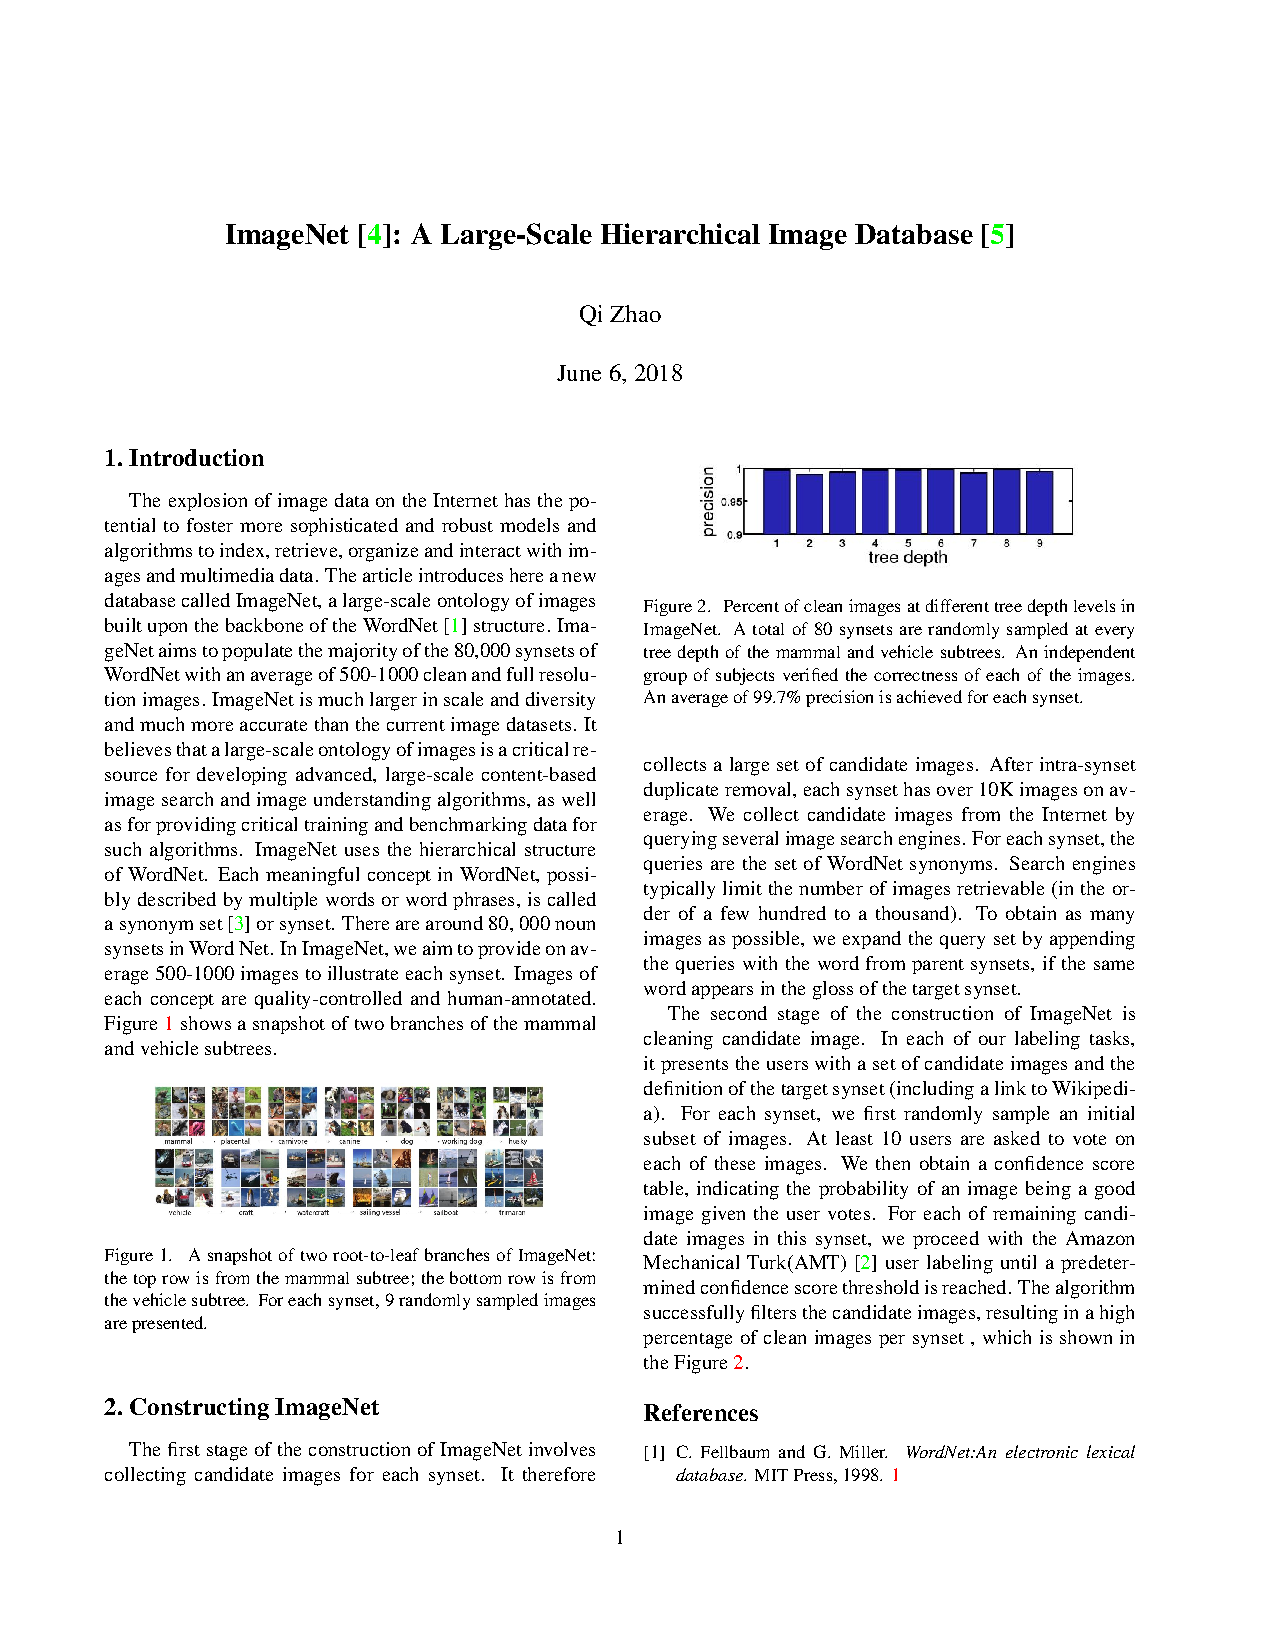
\includegraphics[width=0.8\linewidth]{ImageNet.JPG}
\end{center}
 \caption{ A snapshot of two root-to-leaf branches of ImageNet: the top row is from the mammal subtree; the bottom row is from the vehicle subtree. For each synset, 9 randomly sampled images are presented.}
\label{fig:long}
\label{fig:onecol}
\end{figure}
\section{Constructing ImageNet}
 The first stage of the construction of ImageNet involves collecting candidate images for each synset. It therefore collects a large set of candidate images. After intra-synset duplicate removal, each synset has over 10K images on average. We collect candidate images from the Internet by querying several image search engines. For each synset, the queries are the set of WordNet synonyms. Search engines typically limit the number of images retrievable (in the order of a few hundred to a thousand). To obtain as many images as possible, we expand the query set by appending the queries with the word from parent synsets, if the same word appears in the gloss of the target synset.
 \par The second stage of the construction of ImageNet is cleaning candidate image. In each of our labeling tasks, it presents the users with a set of candidate images and the definition of the target synset (including a link to Wikipedia). For each synset, we first randomly sample an initial subset of images. At least 10 users are asked to vote on each of these images. We then obtain a confidence score table, indicating the probability of an image being a good image given the user votes. For each of remaining candidate images in this synset, we proceed with the Amazon Mechanical Turk(AMT)~\cite{Irani2017Amazon} user labeling until a predetermined confidence score threshold is reached. The algorithm successfully filters the candidate images, resulting in a high percentage of clean images per synset , which is shown in the Figure~\ref{fig:short}.
\begin{figure}[t]
\begin{center}
\includegraphics[width=0.8\linewidth]{ImageNet1.JPG}
\end{center}
 \caption{ Percent of clean images at different tree depth levels in ImageNet. A total of 80 synsets are randomly sampled at every tree depth of the mammal and vehicle subtrees. An independent group of subjects verified the correctness of each of the images. An average of 99.7\% precision is achieved for each synset.}
\label{fig:long}
\label{fig:short}
\end{figure}


{\small
\bibliographystyle{ieee}
\bibliography{24}
}


\end{document}

